%The supply chain of the dairy genetics markets comprises two parts; the first is animal breeders, whose objective is to breed the best bulls (those with the highest breeding values). The second part is the genetics companies that sell the semen from those bulls to commercial dairy farmers, who choose which animal to buy based on his trait levels and pedigree.

%Genetic improvement occurs only in the first part, where bulls and cows are selected to breed the next generation of animals. The most common method breeding method is called \textbf{linebreeding}. Linebreeding is mating individuals related to a common ancestor to maintain a substantial relationship with this animal while keeping inbreeding levels at an "acceptable" rate. These matings are usually called "elite matings" and are performed by animal breeders within their herds; on the other hand, breedings within dairy farmers' herds are called "normal matings" because their sole purpose is to give birth to milk cows and are usually performed using sexed semen\footnote{Sexed semen contains an enriched proportion of X chromosome-bearing sperm cells to maximize the likelihood of giving birth a female animal.}.

%Animal breeders and genetics companies compete to offer an animal with the highest trait values, which provides the best possible improvement over the cohort's average. But, as breeders continue to expand the supply of more demanded lines, the average degree of relatedness of all animals in the market grows, which leads to detrimental effects in the long run. On the other side of the market, dairy farmers want highly productive cows, so they are willing to pay a premium for the genetics from the "best" bulls.    

%The demand for cattle genetics is made up of all dairy farmers in the US and abroad who periodically buy bull semen to impregnate their cows for two reasons: a cow needs to be pregnant or weaning her calf to produce milk, and also because they are going to need new cows in the upcoming years; a cow’s productive life is about four years. Dairy farmers rarely keep bulls within their herds because they do not contribute to their profits, so genetics companies provide the semen to impregnate cows. On the other hand, the supply of dairy genetics is constituted by genetics companies that breed bulls to meet the demand for specific traits. To do so, they choose sires and dams with a particular objective. By doing so, they ensure that the next generation of bulls will have a similar or higher level of traits.

%Selective breeding is the only way to carry out directional genetic change \citep{Melton_Heady_Willham1979}; by doing so, breeders decide which bulls mate with a specific cow to produce the next generation of animals whose semen will be marketed to dairy farmers, who are interested only in cows, since every all production traits (e.g., milk and protein content) are expressed in females only. 

%The bovine genome was sequenced in 2008 \citep{Bovine2009}, providing animal breeders with the last missing piece required to make genomic selection commercially viable; the "50K" chip was released that same year, a commercial system that simultaneously detects up to 50,000 SNPs, thus kickstarting the genomic selection era. Genomic testing of young bulls immediately decreased the generation interval (average age of parents when their select offspring is born). It accelerated the genetic gains (variation in breeding values per year) for North America's dairy cattle population \citep{Guinan2023}. 


%\cite{Melton_Heady_Willham1979, Melton1994} describe a breeder's decision problem as a profit-maximizing firm that combines exogenous inputs ($x_{i}$, $i=1,\dots, m$) and genetic inputs ($g_{j}$, $j=1,\dots, n$) to produce a bull $y$ in a production function $f(.)$ to maximize profits for given bull prices ($p$), and input costs ($w_{i}$ and $r_{j}$), then the profit function is:

%\begin{equation}
%    \pi^{breeder}=pf(x_{1},\dots,x_{m},g_{1},\dots,g_{n})-\sum_{i=1}^{m}w_{i}x_{i}-\sum_{j=1}^{n}r_{j}g_{j}+\sum_{j=1}^{n}\lambda_{j}(\mu_{j}-g_{j})
%\end{equation}

%The last part reflects that breeders profit from supplying animals that perform better than the average trait level for the breed in a given period. Then we define $\mu_{j}$ as the average of trait $j$ across all animals ($N$) in the market at a given period:

%\begin{equation*}
%    \mu_{j}=\sum_{i=1}^{N}g_{ij}f(g_{ij})
%\end{equation*}

%$f(g_{j})$ is the distribution of trait $j$. A breeder will be paid a premium if his animal offers a degree of improvement over the average for the trait, and this is evident from the first-order conditions:

%\begin{eqnarray*}
%    \dfrac{\partial \pi}{\partial x_{i}} &=& p\dfrac{\partial f}{\partial x_{i}}-w_{i} = 0\quad i=1,\dots,m\\
%    \dfrac{\partial \pi}{\partial g_{j}} &=& p\dfrac{\partial f}{\partial g_{j}}-r_{j}-\lambda_{j} = 0\quad j=1,\dots,n\\
%    \dfrac{\partial \pi}{\partial \lambda_{j}} &=& \mu_{j}-g_{j}=0\quad j=1,\dots,n\\
%\end{eqnarray*}

%The sign of the lagrangian constraint depends on the difference between the breed average for trait $j$ and the trait value for the bull $g_{j}$. If a breeder cannot supply an improvement over the breed average, then the marginal cost of trait $j$ will be higher:

%\begin{equation}
%  p\dfrac{\partial f}{\partial g_{j}}=r_{j}+\lambda_{j}  
%\end{equation}

%Achieving a marginal change in the mean level of a trait $j$ is worth $-\lambda_{j}$ in terms of additional profits. Similarly, we can interpret $\lambda_{j}$ as the Karush-Kuhn-Tucker condition that $\lambda_{j}>0$ if and only if $\mu_{j}-g_{j}>0$ and $\lambda_{j}=0$ otherwise, that is, this parameter is the shadow price of genetic gains\footnote{As \cite{Melton1994} point out, $\dfrac{\partial\pi}{\partial\mu_{j}}=\lambda_{j}$ is the effect on profits of a marginal increase in the population mean of trait $j$}. Breeders compete with each other to maximize profits; to do so, they will attempt to release into the market a bull with the highest possible trait values $g_{j}$. 

%Typically, breeders do not select animals based on a single trait value but as a weighted average of those traits, using what is known as a \textbf{selection index} \citep{Hazel1943}, where the magnitude of each weight is a measure of the importance of the trait in the context of a breeding program. Throughout this paper, we argue that most breeders have one objective: to maximize the value of an index because the higher its value, the higher the price of an animal will be.

%In other words, let $I$ be a selection index with weights $\omega_{j}$, then its value will be:

%\begin{equation}
%    I(\mathbf{g}) =\sum_{j=1}^{k}\omega_{j}g_{j}
%\end{equation}

%With $\sum_{j}\omega_{j}=1$ and $k\leq n$. A selection index summarizes the information from a set of $k$ genetic traits, and it is used to rank bulls so that top-ranked animals sell their genetics at a higher price. Breeders are suppliers of genetic improvement to dairy farmers.

%\subsection{Modeling dairy farmers\label{subsec:demand}}

%Dairy farmers demand genetics to improve their productivity in the next period by choosing the bulls with the best characteristics. However, the traits that constitute an animal are marketed as a "bundle" of traits embedded in each animal. Keeping our notation from the last section, let $g_{j}$, $j=1,\dots,n$ be the set of genetic traits, define $G(g_{1}, g_{2}, \dots,g_{n})$ be the set of traits that defines a bull \citep{Kerr1984}, then the farmer's production function is:

%\begin{equation*}
%    y = f(x_{1}, \dots, x_{m};G(\mathbf{g}))
%\end{equation*}

% Show how farmers don't care about inbreeding, only trait levels!

%Where $x_{i}$ is the level of non-genetic input $i$ and $G$ is the genetic value of the bull chosen based on their genetic traits and the animal's price, then the farmer's profit function is:

%\begin{equation*}
%    \pi^{farmer} = p_{m}f(x_{1}, \dots, x_{m};G(\mathbf{g}))-\sum_{i=1}^{n}w_{i}x_{i}-pG(\mathbf{g})
%\end{equation*}

%$p_{m}$ is the price of their output (gallons of milk, for example), $p$ is the price of bull genetics paid by the farmer, and $w_{i}$ is the price of non-genetic input $i$. The most salient characteristic of this profit function is that $G(\mathbf{g})$ is discrete since there are only a limited number of options available, then:

%\begin{equation*}
%    \dfrac{d\pi^{farmer}}{dG} = p_{m}\dfrac{\partial f}{\partial G}-p = \sigma
%\end{equation*}

%The economic value of an animal's genome can be obtained by totally differentiating $\pi^{farmer}$ with respect to the inputs and $G(.)$. Still, this term is not equal to zero, so $p+\sigma$ is the maximum willingness to pay for a bull's genetics, and $\sigma$ is the opportunity cost of buying a specific animal's genetics. In our case, the value of $\sigma$ is a decreasing function of the rank of an animal; the higher ranked an animal is, the lower the opportunity cost of his genetics.

%\begin{equation*}
%    p_{m}\dfrac{\partial f}{\partial G} = p+\sigma
%\end{equation*}

%$G(\mathbf{g})$ is an index of embodied characteristics, and it is assumed to be linearly homogeneous, hence:

%\begin{equation*}
%    pG(\mathbf{g}) =\sum_{j=1}^{n}p\dfrac{\partial G}{\partial g_{j}}g_{j}=\sum_{j=1}^{n}p_{j}g_{j}
%\end{equation*}

%Where $p_{j}$ is the implicit price of trait $j$, this is the main result from the \textbf{Input Characteristics Model} of \cite{ladd1976}, and each price is equal to the market price a trait would have if it could be marketed independently. 

%\subsection{Genetic improvement\label{subsec:genetic_improvement}}


%\begin{equation*}
%    \text{selection intensity} = \dfrac{\overline{g}^{s}_{t}-\mu}{\sigma_{y}}
%\end{equation*}

%\begin{equation}
%    \Delta g_{t+1} = \dfrac{h^{2}}{L}\left(\overline{g}^{s}_{t}-\mu\right)\label{eq:2}
%\end{equation}

%$\Delta g_{t+1}$ is the genetic progress in a single generation of selection. Selection intensity and genetic variation are inversely proportional to the generation interval; the generation interval is the time required to replace one generation with the next; the shorter the interval, the faster the genetic change. In other words, genetic improvement is driven by two forces: selection intensity and generation interval. An increase in selectivity or a decrease in the generation interval increases genetic gains per generation.

%The Breeders' equation (equation \ref{eq:2}) explains the trends we observe in the genetic traits. A positive selection intensity makes traits have an upward trend\footnote{SCS has a downward trend because a lower value implies that cows are less likely to suffer from infection of their udders.} on average every year. Still, genomic selection shortened the generation interval ($L$), thus increasing the rate of change further.

%Then, the selection of better animals has two effects. First, it increases the average level of a trait due to truncation of the distribution of traits by culling "inferior" individuals; second, it also lowers the variance of any given trait; this is called the "Bulmer effect," and it is a consequence of the truncating distribution of traits.

%\subsection{Inbreeding Depression\label{inbreeding}}


%American Holstein cattle have experienced the deleterious effect of such abnormalities; a bull called \textit{Pawnee Fram Arlinda Chief}, born in 1962, had an undesirable that caused his descendants to have a lower conception rate and a higher frequency of neurodevelopmental disorders, which caused about 525,000 spontaneous abortions, accounting for \$ 420 million in losses for the dairy industry \citep{Adams2016}.

%In the case of polygenic traits (traits that are a consequence of the interaction among several genes), these effects are individually minimal but, in the aggregate, can have a significant negative impact on the expression of a trait; this is known as \textbf{inbreeding depression}, the result of a poor gene combination value.

%Inbreeding depression is a consequence of inbreeding, but the reverse does not hold; mating closely related animals is a common way to ensure that the next generation will have similar traits to their parents. Furthermore, \cite{Falconer1996} show that the average level of a trait and the level of inbreeding is not linear if there are interactions between loci (positions on a  specific chromosome where  a gene is located.) Consequently, an increase in the level of inbreeding does not necessarily imply a higher likelihood of inbreeding depression, but as the population becomes more inbred, it will be the case.

%Inbreeding is commonly measured using the \textbf{Inbreeding Coefficient} ($F_{X}$) \citep{Wright1922}, defined as the probability that two alleles\footnote{Alternative forms of a gene, inherited from the sire, the dam or both.} in an individual were both descended from a single allele in an ancestor.

%\begin{equation}
%        F_{X}=\sum_{ca=1}^{K}\left(\dfrac{1}{2}\right)^{n_{1}+n_{2}+1}(1+F_{ca})
%\end{equation}

%Where $ca$ denotes the common ancestor, $n_{j}$ is the number of generations separating the common ancestor from the sire (dam), and $F_{ca}$ is the inbreeding of the common ancestor.

%\begin{figure}[H]
%\centering
%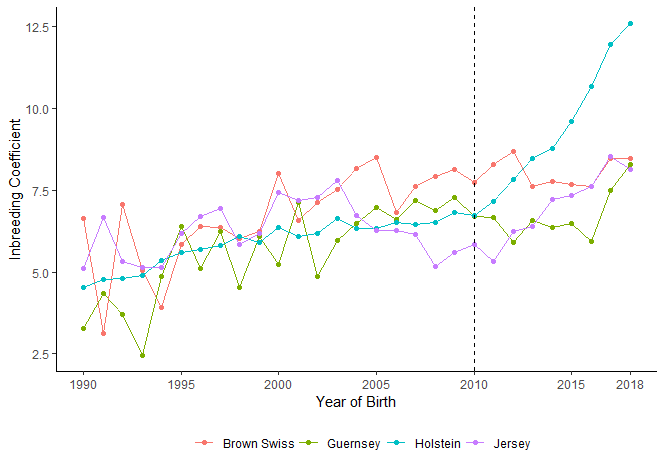
\includegraphics[width=16cm]{figures/Inbreeding.png}
%\caption{Average inbreeding rate by bull's generation and breed}
%\label{fig:inb}
%\end{figure}

%Figure \ref{fig:inb} shows how the inbreeding rate by breed has changed since 1990; among most dairy breeds, Holstein bulls stand out as the breed where inbreeding has increased at a higher rate since 2010, followed by Jersey and Guernsey bulls.

%\subsection{The North American cattle genetics market\label{subsec:genetics_market}}

 

%For example, the development of artificial insemination in 1938 and freezing technology for bull semen in 1953 brought into existence a group of animals we call ``Superstar Sires", bulls who have fathered thousands of daughters because of their superior genetics and gave birth to the three dominant pedigrees of the present day, namely those of "Pawnee Farm Arlinda Chief," "Round Oak Rag Apple Elevation," and "Penstate Ivanhoe Star." \citep{Hutchins_Hueth2023} 

%Two (exogenous) technological innovations in the 20$^{th}$ century led to a significant decrease in the male diversity of Holstein cattle\footnote{The Holstein or Holstein-Friesian breed, originated in the present-day Netherlands and it is the most widespread dairy cattle breed in North America since it was introduced in 1852.}. According to \cite{Yue2015}, all Holstein bulls in North America are descendants of two bulls imported from the Netherlands in 1880: "Neptune H" and "Hulleman."

%Figure \ref{fig:inb_prod} shows the relationship between inbreeding and production traits (milk yields, percent of fat in milk, and pounds of protein in milk) split between three periods, pre-2009 (before genomic selection), 2010-2015, and 2015-2020, and by the status of the animal\footnote{"Active" means that the animal's traits were tested on his daughters, "Genomic" implies that they were tested through the bull's genome, "Foreign," means that the animal was tested outside the United States.}. 

%\begin{figure}[H]
%    \centering
%    \includegraphics[width=16cm]{figures/inb_prod.png}
%    \caption{Production trait values for Holsteins as a function of inbreeding rate\\ \small \textbf{Source}: NAAB}
%    \label{fig:inb_prod} 
%\end{figure}

%The relationship between production trait levels increases with the inbreeding rate, as animals are partially selected for them. The strength of the relationship varies with inbreeding levels; for values between 0.05 and 0.15, there is a positive relationship between inbreeding and average values of the three traits. However, as inbreeding levels increase, the strength begins to plateau.

%However, as inbreeding rates continue to increase, inbreeding depression becomes a concern \citep{Cole2019}, regarding fertility traits. Figure \ref{fig:inb_fert} shows the relationship between the inbreeding rate and three fertility traits: Daughter Pregnancy Rate (DPR), the percent of nonpregnant cows that become pregnant during 21 days; Cow Conception Rate (CCR), the percentage of inseminated cows that become pregnant each insemination; and Heifer Conception Rate (HCR), the percent of inseminated heifers that become pregnant after each insemination. The Daughter Pregnancy Rate measures how easy it is for the bull's daughters to become pregnant. In contrast, cow and heifer conception rates measure how likely a cow or a heifer will become pregnant by artificial insemination. Fertility traits are the ones more likely to be affected by inbreeding depression. Still, the plot doesn't hint at apparent effects other than a higher average inbreeding rate across periods and genomic-proven bulls having more variability in most traits than daughter-proven bulls.


%Productive Life measures the animal's longevity as how much a cow is expected to produce milk. Somatic Cell Score is a proxy for udder health; a high SCS indicates that the cow suffers from mastitis (intramammary infection). Finally, milk, protein, and fat yield are measures of how productive the bull's daughters are expected to be in terms of the quality of their milk. Our data shows similar trends as shown by \cite{garciaruiz2016}; there is significant evidence of a change in the rate of change of all traits after the introduction of genomic selection, except for the daughter pregnancy rate, which appears to show signs of a reversal in its rate of change from 2016 onwards.

%\begin{figure}[H]
%    \centering
%    \includegraphics[width=16cm]{figures/inb_fert.png}
%    \caption{Fertility traits for Holsteins as a function of inbreeding rate\\ \small \textbf{Source}: NAAB}
%    \label{fig:inb_fert} 
%\end{figure}



%Similarly, the strength of the tie between two animals is a function of their degree of relatedness; for example, a sire and his son share 50\% of their genotype, so their relationship coefficient is $1/2$, for a grandsire and his grandson is $1/4$.

%\newpage
%\subsection{Selection\label{subsec:selection}}

%Selection, also called ``Selective Breeding,'' is the only way by which breeders make directional genetic change \citep{Melton_Heady_Willham1979}; by doing so, they decide which bulls mate with a specific cow to produce the next generation of animals whose semen will be marketed to dairy farmers, who are interested only in cows, since every all production traits (e.g., milk and protein content) are expressed in females only.

%Animal selection is carried out in the context of a breeding program, a description of a goal or set of goals (breeding objectives) that a breeder wants to pursue, defined in terms of qualitative characteristics, such as coat color or lack of horns, or quantitative traits, such as fat content of milk or weaning weight \citep{Bourdon2000}. When there are several breeding objectives, the selection is usually carried out using a \textbf{Selection Index} \citep{Hazel1943}, where the expected value of each trait is multiplied by a constant between zero and one, the larger the value of each constant, the more influential the weight of a particular feature.

%The \textbf{Total Performance Index} (TPI) is a selection index used by the Holstein Association of the United States of America and can be used to show the overall effects of increased selection. Figure \ref{fig:tpi} shows a change in the trend starting in 2010 but leveling after 2018.

%\begin{figure}[H]
%    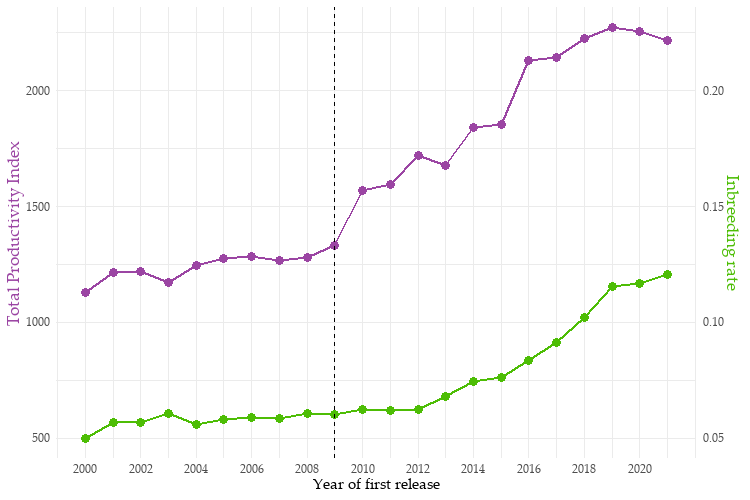
\includegraphics[width=\textwidth]{figures/tpi.png}
%    \caption{Average Total Performance Index of Holstein bulls\\ \small \textbf{Source}: NAAB}
%    \label{fig:tpi} 
%\end{figure}


%\subsection{Effects of Genomic Selection\label{subsec:genomic_selection}}

%With genomic testing, it is no longer necessary to wait for the bull's progeny to grow since an animal can be tested as soon as it is born for the presence of specific traits on its genome. Consequently, the generation interval, the average age of parents when offspring are born \citep{Wiggans2022}, has decreased from around 5.5 years to less than two years, close to the biological minimum. 

%\begin{figure}[H]
%    \centering
%    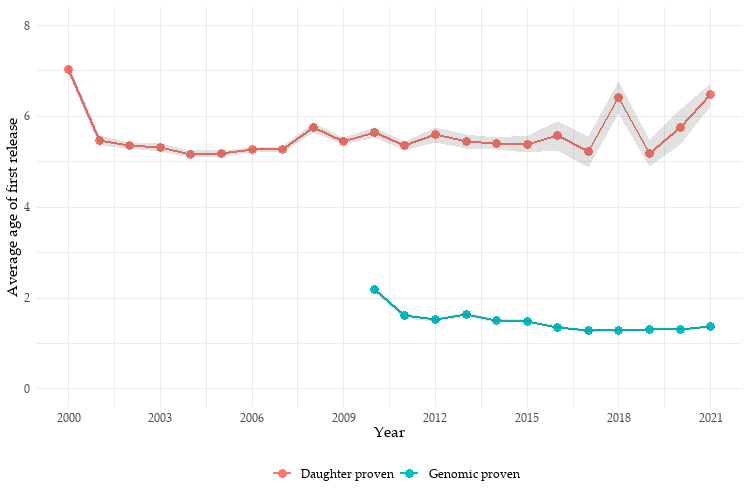
\includegraphics[width=16cm]{figures/generation_interval.png}
%    \caption{Average age at first proof for Holstein bulls\\ \small %textbf{Source}: NAAB}
%    \label{fig:gen_int} 
%\end{figure}


%\begin{equation}
%    y_{i}=\mu + a_{i}+c_{i} + e_{i}
%\end{equation}

%Where:
%\begin{description}
%    \item[$y_{i}$]: phenotypic value of a trait belonging to animal $i$.
%    \item[$\mu$]: population average of that trait.
%    \item[$a_{i}$]: breeding value.
%    \item[$e_{i}$]: environmental factors that affect the animal's response.
%\end{description}

%Breeding values are inherited directly from the animal's parents and are equal to the sum of additive effects within and across loci (fixed positions within a chromosome). These values can be estimated and predicted based on the animal's observed values, such as age, ancestry, sex, and other variables. On the other hand, gene combination values result from a set of interactions across different parts of the genotype; this makes them non-predictable or estimable. Therefore, their effect is usually incorporated into the error term of a linear model.

%The breeding value is then:

%\begin{equation}
%    a^{offspring}_{i} = \dfrac{1}{2}a^{sire}_{i}+\dfrac{1}{2}a^{dam}_{i}+\delta_{i}
%\end{equation}

%Where $a^{sire}_{i}$ and $a^{dam}_{i}$ are the breeding values of the animal's parents, $\delta_{i}$ is a random component called \textbf{Mendelian sampling} since each offspring receives a random sample of their parent's alleles. Half the breeding value of a parent is also called the animal's \textbf{Transmitting Ability}.

%\subsection{Estimation of breeding values}

%Breeding values are not directly observable but can be estimated from the data as a random effects model \citep{Rosa2020}:

%\begin{equation}
%    y_{i}=\mu + a_{i} + \epsilon_{i}
%\end{equation}

%Then, the predicted value for $a_{i}$, called the \textbf{Expected Breeding Value}\footnote{If we divide the number by two, we get the \textbf{Predicted Transmitting Ability} (PTA) for trait $y$} and is equal to:

%\begin{equation}
%    \widehat{a}_{i} = h^{2}\times (y_{i}-\mu)
%\end{equation}

%$h^{2}$ is called the \textbf{Heritability} of trait $y$ and is the fraction of the phenotypic variance that is explained by additive genetic effects:

%\begin{equation}
%    h^{2}=\dfrac{\sigma^{2}_{a}}{\sigma^{2}_{y}}
%\end{equation}

%Heritability is assumed to be a constant population parameter estimated from the data. It is equal to the coefficient of determination of the regression of phenotypical values on breeding values. 



%Perhaps the closest analogy is the market for seeds; in that market, seed companies develop new varieties based on farmer's demand, such as glyphosate or drought tolerance, and then sell seeds to farmers who plant them. Seed companies then developed genetically engineered traits subject to copyright law, thus forcing farmers to sign restrictive retailing contracts to replant those seeds in further seasons \citep{Ciliberto2019}. 

%The dairy genetics industry works similarly when a dairy farmer buys semen; they expect to obtain a female. However, if that is not the case, the genetics company usually has the right to buy back the calf to avoid being outbid by a competitor.

%Technology adoption is usually modeled as a slow-moving process \citep{Hall2003} resulting from aggregating several individual decisions depending on each decision maker's information, uncertainty, and cost structure. Thus, adoption patterns tend to follow an S-shaped curve \citep{Griliches1957}, where a relatively small number of agents adopt the new technology first, but as time progresses, more and more people adopt it. It grows exponentially until it reaches 100\%. 

%This is not the case, and the high starting costs for genotyping can easily explain it since large companies were the ones that could initially afford it. Still, since the cost decreased quickly, more and more companies could genotype their calves. Figure \ref{fig:percent_size} breaks down the adoption percent by firm size; larger firms genotyped a more significant percent of their newborn calves in 2010, and the share has grown steadily, while smaller firms followed them at a slower rate.


%We can look closely at those companies to distinguish which had the most significant number of bulls released into the market from 2010 on; in figure \ref{fig:new_bulls_large}, we show the six larger firms, while figure \ref{fig:new_bulls_size} shows only the six largest "small" firms. In the case of the large firms, Select Sires and Semex Alliance explain the bulk of the increase in 2010.

%\begin{figure}[H]
%     \centering
%     \begin{subfigure}[b]{\textwidth}
%         \centering
%         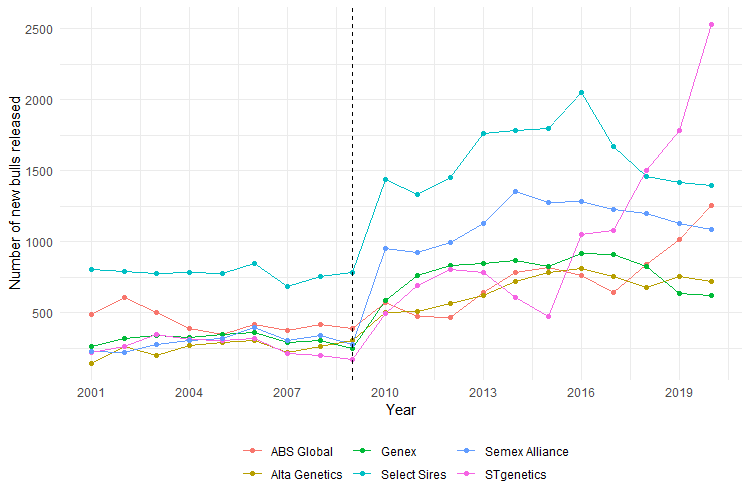
\includegraphics[width=\textwidth]{figures/new_bulls_large.png}
%         \caption{Large firms}
%         \label{fig:new_bulls_large}
%     \end{subfigure}
%     \hfill
%     \begin{subfigure}[b]{\textwidth}
%         \centering
%         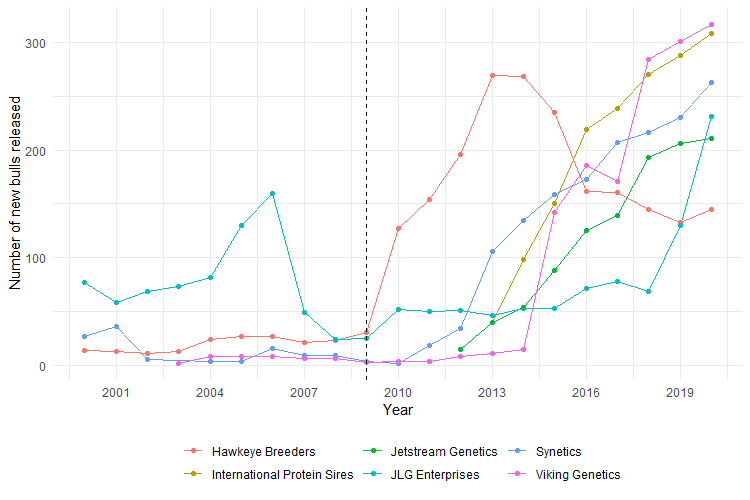
\includegraphics[width=\textwidth]{figures/new_bulls_small.png}
%         \caption{Small firms}
%         \label{fig:new_bulls_small}
%     \end{subfigure}
%        \caption{Number of genotyped bulls by firm and size\\
%        \small \textbf{Source}: NAAB}
%        \label{fig:new_bulls_size}
%\end{figure}

%Smaller firms, in turn, generally adopted genomic testing later, and in smaller numbers, except "Hawkeye Breeders" which also increased threefold the number of bulls released in 2010. 

%\section{Productivity growth in the dairy industry}
%A more nuanced view of biological processes is using a neoclassical production function where a unit of output (milk) is a function of a set of $n$ inputs and an index of $p$ genetic traits:

%\begin{equation}
%    y = f(x_{1}, x_{2}, \dots, x_{n}, G(a_{1}, \dots, a_{p}))
%\end{equation}

%To simplify the  exposition, assume for the moment that there is only one single trait relevant for milk production, $a$:

%\begin{equation}
%    y = f(x_{1}, x_{2}, \dots, x_{n}, G(a))
%\end{equation}

%Then, we now calculate the derivative of $y$ with respect to time:

%\begin{equation}
%    \dfrac{dy}{dt}= \sum_{i=1}^{n}\dfrac{\partial f}{\partial x_{i}}\dfrac{dx_{i}}{dt}+\dfrac{\partial f}{\partial G}G'(a)\dfrac{da}{dt}
%\end{equation}

%Dividing by $y$ and multiplying and dividing by $x_{i}$ and $a$:

%\begin{equation}
%    \dfrac{dy/dt}{y}= \sum_{i=1}^{n}\dfrac{\partial f}{\partial x_{i}}\dfrac{x_{i}}{y}\dfrac{dx_{i}/dt}{x_{i}}+\dfrac{\partial f}{\partial G}G'(a)\dfrac{a}{y}\dfrac{da/dt}{a}
%\end{equation}

%Assuming that the firm maximizes profits, we have that $\frac{\partial f}{\partial x_{i}}=\frac{w_{i}}{p}$, where $w_{i}$ is the price of factor $i$ and $p$ is the price of a gallon of milk, then:

%\begin{equation*}
%    \dfrac{\partial f}{\partial x_{i}}\dfrac{x_{i}}{y}=\dfrac{w_{i}x_{i}}{py}=\dfrac{w_{i}x_{i}}{C(w_{1}, \dots, w_{n}, y)}=\theta_{i}
%\end{equation*}

%Finally, define the rate of change in $x_{i}$ as : $\hat{x}_{i}=\frac{dx_{i}/dt}{x_{i}}$ so that:

%\begin{equation*}
%    \hat{y} = \sum_{i=1}^{n}\theta_{i}\hat{x}_{i}+\theta_{G}G'(a)\hat{a}
%\end{equation*}

%If we keep all other factors constant, the equation linking genetic change to milk output is:

%\begin{equation}
%    \hat{y} = \theta_{G}G'(a)\hat{a}
%\end{equation}

%Where:

%\begin{equation*}
%    \hat{a} = \dfrac{h}{t}\left(\dfrac{a^{P}-\mu_{P}}{\sigma_{y}}\right)\sigma_{a}
%\end{equation*}

%Therefore, genetic gains are translated into higher milk output, provided that $G'(a)>0$; the trait positively impacts the Genetic index. Note that this can be straightforwardly generalized to $p$ traits. $\theta_{G}$ is the share of genetics in the total cost of a dairy firm.

%\input{milk_output}



%\section{Consequences of Genomic Selection}
%The most relevant technological breakthrough of the last 20 years in the animal breeding industry is genomic sequencing; before this technology, a bull needed to have at least one generation of daughters to be "proven," that is, tested for the level of a specific trait. Bulls need to be tested because due to \textbf{epistatic} effects, production traits are not expressed in male animals\footnote{Or, in layman's terms, "bulls can't be milked".}. Now, because of genomic evaluation, we can test an animal for the presence of traits as soon as he is born, at the expense of a lower precision (95\% for daughter proven versus 70\% for genomic-proven bulls), but this is enough for farmers to select bulls.

%The most important consequence of this technology is that now generation intervals are cut by half, thus increasing the response to selection by 50\%; in the selection equation, $L$ decreases by half, but since it enters the selection equation in the denominator, the entire term is multiplied by 2.

%Genomic testing is carried out by testing for genetic markers, parts of the DNA molecule that can be identified in individuals; they can be close to a gene of interest and, thus, select for a favorable version of such gene. Genes that control a quantitative trait are called \textbf{Quantitative Trait Loci} (QTL). However, most traits are not controlled by a single gene, but by a combination of them, and recently the cost of sequencing a genome has made it possible to obtain many markers, regardless of their effect size. The most widely used type of marker is the \textbf{Single Nucleotide Polymorphism} (SNP), which marks the place in the genome in which there is a variation in a single nucleotide\footnote{A DNA molecule is comprised of a combination of four nucleotides: Adenine, Cytosine, Thymine and Guanine, an SNP is a single change of one of such nucleotides for another in a specific locus.}.

%In this context, breeding values can be predicted based on measured data from $n$ animals that are sequenced for the presence of 50,000 SNPs, each being a categorical variable with three values ($AA$, $A$a, and $aa$, as shown in a Punnett Square) coded as either (-1, 0, 1) or (0,1,2), then the model is:

%\begin{equation}
%    y = \mu+\beta_{1}x_{1}+\dots+\beta_{50,000}x_{50,000}
%\end{equation}

%Usually $n<50,000$, this model has to be estimated using a variable selection method such as Ridge Regression or LASSO or Bayesian Methods with a shrinkage prior distribution. Then, the Expected breeding value is:

%\begin{equation*}
%    \hat{a} = \hat{\mu}+\hat{\beta}_{1}x_{1}+\dots+\hat{\beta}_{k}x_{k}
%\end{equation*}

%The main disadvantage of this method is that the association of SNPs with traits disappears quickly in a few generations because the link between SNPs and the genes associated with the trait disappears due to selection. Hence, they have to be re-estimated when new generations become available.

%Let $i$ be a line that is the set of bulls that have a common ancestor, which belongs to one of two groups $k\in \left\lbrace treat,control\right\rbrace$, which has $n_{it}$ animals being born in any year $t$ (cohorts), each with its inbreeding rate $F_{it}$, and let $j$ be any animal in a cohort born during year $t$, then the average inbreeding rate of family $i$ at year $t$ is:

%\begin{equation}
%    \overline{F}_{it}^{k}= \dfrac{1}{n_{t}}\sum_{j=1}^{n_{t}}F_{ijt}^{k}
%\end{equation}

%The Holstein Association of the United States\footnote{\url{https://www.holsteinusa.com/pedigree_info/calc_details.html}} uses a simple formula to adjust PTAs of several traits by inbreeding rates:

%\begin{equation}
%    \overline{PTA}^{k}_{i} = PTA^{k}_{i}+(\alpha^{k}*F_{i})
%\end{equation}

%$\overline{PTA}^{k}_{i}$ and $PTA^{k}_{i}$ are the corrected and uncorrected predicted transmitting ability of trait $k$ for animal $i$, $\alpha_{k}$ is a trait-specific constant and $F_{i}$ is the inbreeding rate of animal $i$. $\alpha_{k}$ is negative to reflect the negative impact of inbreeding on fertility.

%Larger genetics companies adopted genomic selection techniques faster because of their high sunk costs. To correctly identify which gene combinations are correlated with specific traits, a significantly large number of animals had to be sequenced first. According to \cite{Vanraden2009}, a first batch of 3576 Holstein bulls was first sequenced in 2008 and used as the ``train set" to identify and predict traits for other 1759 bulls that constituted the ``test set'' for the statistical methods used to capture the relationship between genes and observed traits.

%This article studies the consequences of introducing genomic selection in the dairy industry. Genomic selection uses data from an animal's entire set of genes (its genotype) to identify which traits are associated with specific combinations of genes as soon as the animal is born. The most critical consequence of genomic selection is a significant increase in the rate of genetic gain, defined as the intergenerational variation in the quantities of a trait. In other words, every new generation of bulls has even better productivity than the previous, and this difference is growing faster. 

% To produce such an animal, the breeder combines a set of inputs that can be split into two groups: a series of inputs exogenously supplied by the producer (labor, feed, capital, veterinary services) and a series of inputs embodied in the animal (traits.) 
% Those inputs are combined on a production function subject to the prices of exogenous inputs (observed) and genetic inputs, whose prices are implicit but can be estimated based on the price paid for a bull's genetics using the hedonic approach \citep{Schroeder1992, Sy1997}.